\chapter{Use Cases}
\section{Industrial IoT in a smart GreenHouse}
The topic discussed is a case study of a project funded by the Tucany Region and concluded in 2019 whose aim was to develop a technological \textbf{greenhouse} having specific objectives:
\begin{itemize}
   \item Monitor drainage waters
   \item Control the root zone in terms of the presence of nutrients and waters
   \item Compare different cultivation substrates
   \item Develop new models based on AI to enable an intelligent control of the greenhouse
\end{itemize}


\begin{figure}[htbp]
   \centering
   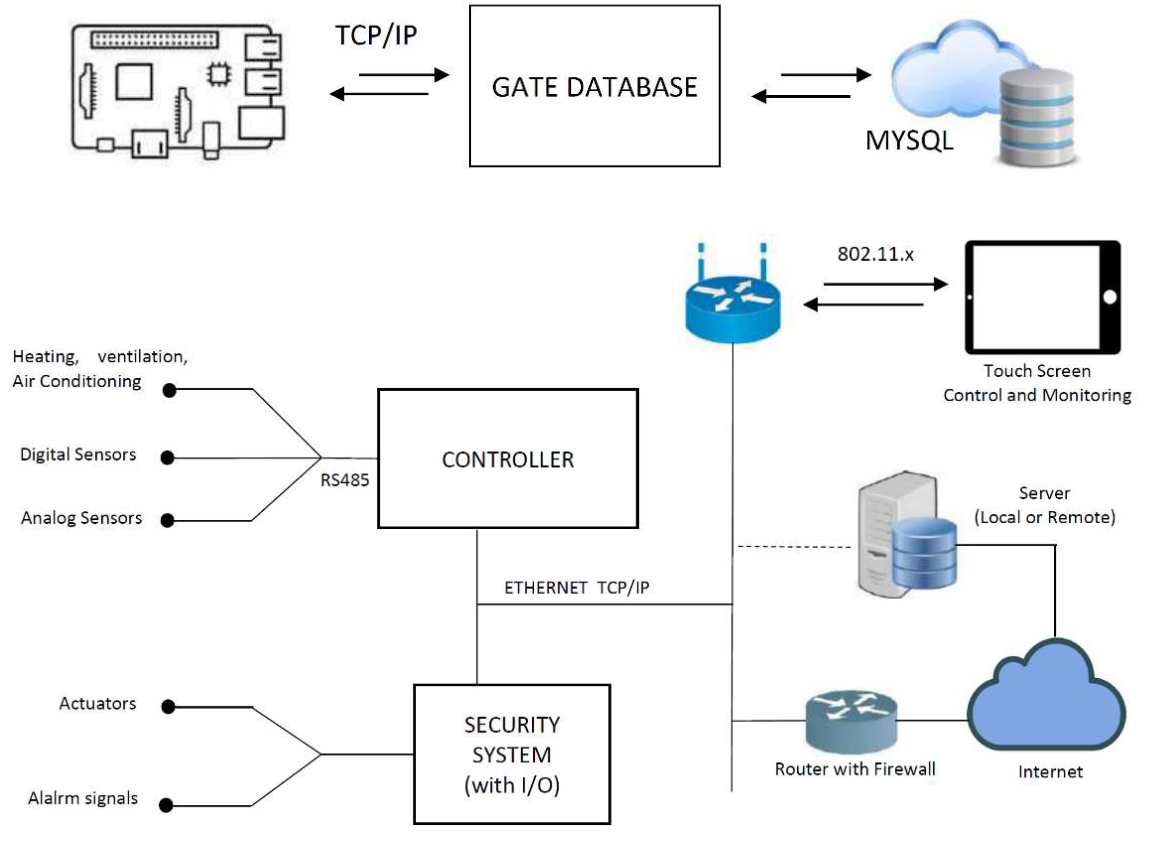
\includegraphics{images/greenhouse_tcp_architecture.png}
   \caption{Greenhouse network architecture}
   \label{fig:greenhouse_tcp_architecture}
\end{figure}
There are some information concerning the architecture and structure of the greenhouse which are not reported here.

The problem is how to analyze data and integrate it with AI;
there are two main aspects:
\begin{enumerate}
   \item 
   Need a control of the installation/systems that goes beyond
   the simple “timed logic”
   \begin{enumerate}
      \item 
      E.g. the fertigation system may need to be controlled
      depending on the actual needs of the crops\dots
      \item \dots that however change with the environmental
      conditions and with their growth
   \end{enumerate}
   \item
   Need to forecast the crops growth to optimize the
   greenhouse (power/water/fertilizers consumption)
\end{enumerate}

The parameters concerning \textbf{crops growth} are:
\begin{itemize}
   \item Leaf area index(LAI)
   \item Dry weight (DW)
   \item Evotranspiration (ET)
\end{itemize}
The idea is to use AI models for growth prediction using a data driven approach.
There a period of data acquisition of $35+52+37$ days (each in a different season) focused on salad.

\begin{figure}[htbp]
   \centering
   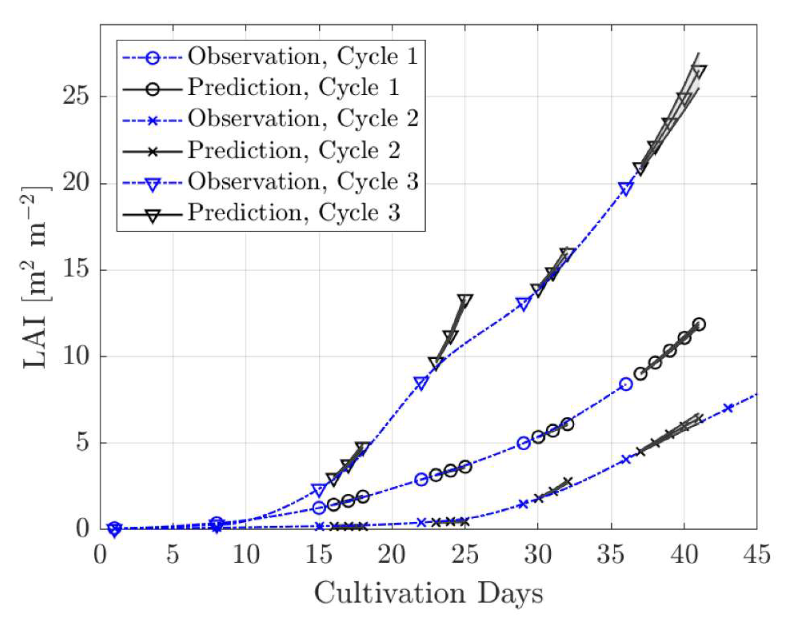
\includegraphics{images/greenhouse_aiprediction.png}
   \caption{Crops growth AI prediction against acquired data}
   \label{fig:greenhouse_aiprediction}
\end{figure}

\section{IoT in Ambient Assisted Living}

The first topic discussed is the \texttt{DOREMI} project, which stands for \textit{Decrease of cOgnitive decline, malnutRition and sedEntariness by elderly empowerment in lifestyle Management and social Inclusion}

\begin{figure}[htbp]
   \centering
   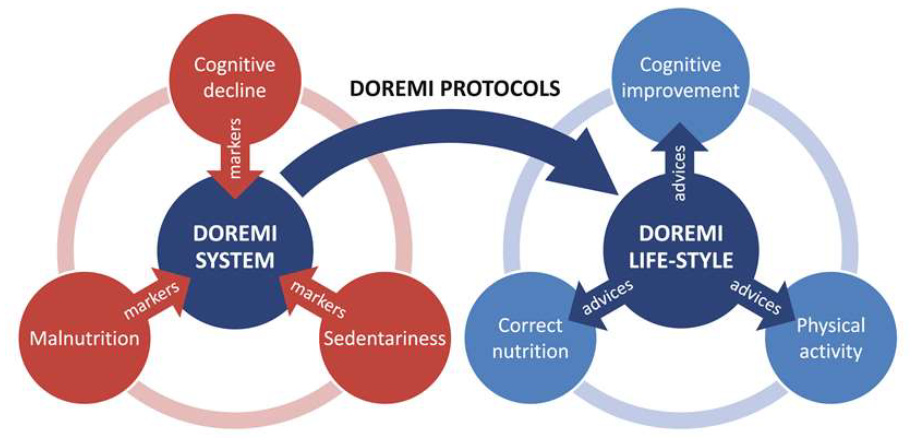
\includegraphics{images/doremi_outline.png}
   \caption{DOREMI project}
   \label{fig:doremi_outline}
\end{figure}

\begin{paracol}{2}
   The idea is to gather data from various sources, in order to obtain a profile of an elder.
   \begin{enumerate}
      \item Wristband
      \begin{enumerate}
         \item assess physical activities, hearth rate, calories
         expenditure, \dots
      \end{enumerate}
         \item Balance board
      \begin{enumerate}
         \item assess user balance according to the Berg scale
      \end{enumerate}
      \item Environmental sensors
      \begin{enumerate}
         \item Indoor localization
         \item Socialization assessment
      \end{enumerate}
      \item App for tablet
      \begin{enumerate}
         \item Enter dietary data
         \item Play cognitive, social, exer-games
         \item Receive feedbacks
      \end{enumerate}
   \end{enumerate}
   \switchcolumn
   \begin{figure}[htbp]
      \centering
      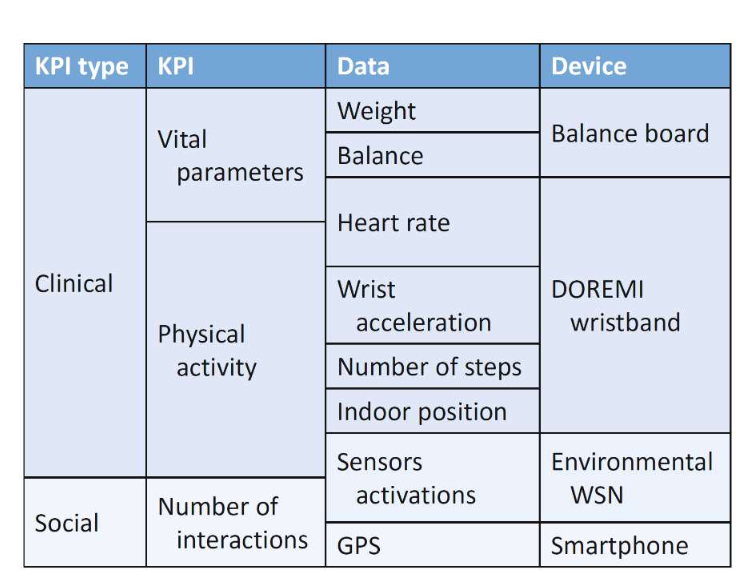
\includegraphics{images/doremi_sensors.png}
      \caption{DOREMI Sensors and related data}
      \label{fig:doremi_sensors}
   \end{figure}

\end{paracol}

\begin{figure}[htbp]
   \centering
   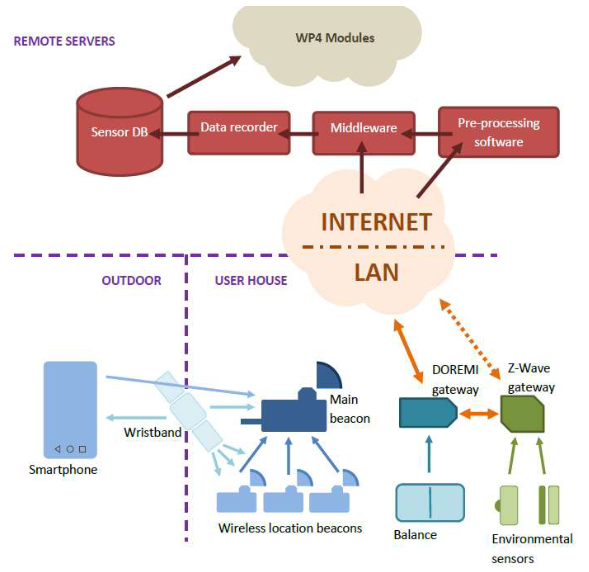
\includegraphics{images/doremi_netarch.png}
   \caption{Wireless sensor network and Cloud architecture}
   \label{fig:doremi_netarch}
\end{figure}

They used chinese Wii Balance Board replicas to asses data on balance and weight of the elder.
Wristbands were needed to measure the Heart Rate, which was later used to establish the calories consumption by applying a Fourier transform to it.

Some sensors instead when activated in a given sequence could indicate a human entering or leaving the house.
Overall about 20 devices per user were used. For the ``pilots'' 400 devices were used in total.

They had to use \ul{two distinct databases}, because some sensors provided time-series data, while more complex ones, such as the balance board, provided measurements.


32 \textbf{pilots} were chosen ranging in 65 to 80 years, half living in Italy and half in the UK, all having 
\begin{itemize}
   \item Mild to moderate cognitive impairment
   \item At risk of malnutrition
   \item Low physical activity
\end{itemize}
The pilots were divided into a \textit{control group} and an \textit{intervention group} made up of 7 and 25 users respectively.

The pilots were forced to follow some rules each day and each, such as wearing the wristband, play the cognitive games, perform suggested exercises etcetera.

\subsection{Human Factor}
When a system is developed for humans it is difficult to predict and handle all possible scenarios.
The human factor in this example impact very much, especially the lack of motivation. 

Other issues were related to inserting the food intake, picking up people spread around Genoa for social meetings, people not wanting sensors in their houses etc.